% (e) Analýza a návrh implementace produktu (včetně diskuse různých alternativ a volby implementačního prostředí).

\chapter{Analýza a návrh implementace}
% Analýza a návrh implementace (včetně diskuse různých alternativ a volby implementačního prostředí).
% Detailní popis uživatele a jeho potřeb.
% Analýzu odkázat na komparativní test.
% Návrh odkázat na low fidelity test.
% V analýze neprezentovat finální řešení ale dopodrobna celý proces.

% TODO kolik času bylo věnováno

Analýza s návrhem probíhaly nezávisle na dvou místech -- po krátké analýze celku a určení vzájemných komunikačních rozhraní byly provedeny analýza s návrhem serverové aplikace a až po jejím dokončení začaly analýza s návrhem mobilní aplikace. V průběhu času jsem se k analýze a návrhu ještě několikrát vrátil a vylepšil / rozšířil to, co se ne vždy na poprvé povedlo.

Analýza se skládala z identifikace potřeb uživatelů, vytvoření případů užití, ze kterých byly odvozeny funkční požadavky, ke kterým byly doplněny nefunkční požadavky. Poté byl vytvořen návrh řešení, zapracován návrh bezpečnosti a celý koncept byl podložen návrhem nasazení. Nakonec byly voleny technologie.

\section{Serverová aplikace}
Začal jsem pracovat nejprve na serverové aplikaci -- jednak na ní měla být ta mobilní závislá (sama na žádné jiné části práce závislá není) a také má užší vazbu ke zpracovávané doméně.


\subsection{Potřeby uživatelů}
Tato část se věnuje potřebám uživatelů serverové aplikace, zejména uživatelů rozhraní, přes které poskytuje informace. Potřeb je mnoho -- proto zde uvedu pouze reprezentativní vzorek.

\subsubsection{Potřeba zjistit informaci}
Potřeba zjistit informaci je základní potřebou, kvůli které se mají uživatelé obracet na systém. Tato potřeba může vzniknout z velikého množství příčin -- od hledání informací spjatých s průchodem studiem, až například po zjišťování jídelního lístku v menze.

\subsubsection{Potřeba ověřit informaci}
Často je cílová skupina uživatelů v situaci, kdy má požadovanou informaci, není si jí ale jistá a potřebuje ji ověřit / vyvrátit. Bez jistoty pravdivosti informace je její hodnota podstatně nižší.

\subsubsection{Potřeba ověřených informací}
Velmi podstatnou potřebou je potřeba ověřených informací. Ačkoliv je název velmi podobný té předchozí, jedná se o dvě diametrálně odlišné potřeby, předchozí se bez naplnění této neobejde. Jakmile jsou informace poskytovány, je nutné, aby byly ověřené -- pravdivé.

\subsubsection{Potřeba aktuálních informací}
Potřeba aktuálních informací opět souvisí s již zmíněnými potřebami -- sebepravdivější jídelní lístek z předchozího dne mi při výběru dnešního oběda bohužel moc nepomůže.

\subsubsection{Potřeba kompletních informací}
Někdy nestačí jen pravdivé a aktuální informace, naopak vědomí záruky pravdivosti a aktuálnosti může i uškodit -- pokud totiž informace nejsou kompletní, může dojít k jejich misinterpretaci a pod vlivem záruk nedojde ke kritickému posouzení. Proto je zde i potřeba kompletních informací.

\subsubsection{Potřeba nalézt, co nehledám}
Na první pohled tato potřeba nedává smysl, v praxi se ale často vyskytují informace, které bychom měli znát a o jejich existenci nemáme ani ponětí. Je proto důležité ve vhodné chvíli sdělit i nepožadované informace, které jsou s velkou pravděpodobností pro adresáta důležité.


\subsection{Případy užití}
Případy užití (\textit{use cases}) jsou takové sekvence kroků, které reprezentují danou činnost prováděnou aktérem na systému a vedou od jejího zahájení až po naplnění.

V serverové aplikaci byli identifikováni celkem tři hlavní aktéři:
\begin{itemize}
 \item Uživatel -- student / softwarová komponenta (\textit{mobilní aplikace}).
 \item Správce -- administrativní pracovník fakulty.
 \item Plánovač -- softwarová komponenta.
\end{itemize}
Roli správce by šlo dále dělit na další role, vzhledem k velmi nízkému rozsahu činností každé z nich (zpravidla jedna činnost), je vše zahrnuto pod tímto souhrnným názvem. Pod plánovačem je zase zahrnut aktér čas.

Uživatel se pouze dotazuje nad systémem a zjišťuje informace. Správce manuálně upravuje informace v systému, může vynutit aktualizaci a jinak spravuje systém. Plánovač automaticky obsluhuje aktualizace obsažených informací.

\subsubsection{UC-S-1: Vyžádání informací}
\subsubsection*{Aktéři:}
\begin{itemize}
 \item Uživatel.
\end{itemize}
\subsubsection*{Systém:}
\begin{itemize}
 \item Serverová aplikace.
\end{itemize}
\subsubsection*{Vstupní podmínky:}
\begin{itemize}
 \item Uživatel zná jazyk dotazovacího rozhraní systému.
 \item Uživatel má přístup k dotazovacímu rozhraní systému.
\end{itemize}
\subsubsection*{Hlavní scénář:}
\begin{itemize}
 \item Uživatel vytvoří dotaz.
 \item Uživatel odešle dotaz na rozhraní systému.
 \item Systém dotaz přijme.
 \item Systém dotaz zpracuje -- nalezne požadované informace.
 \item Systém odešle odpověď.
 \item Uživatel přijme odpověď.
 \item Uživatel zpracuje odpověď.
\end{itemize}
\subsubsection*{Alternativní scénáře:}
\begin{itemize}
 \item V případě neplatného dotazu je navráceno chybové hlášení.
 \item V případě chyby serveru je navráceno chybové hlášení.
\end{itemize}
\subsubsection*{Poznámky:}
\begin{itemize}
 \item V případě nenalezení informace je navrácena prázdná množina.
 \item Pokud je uživatelem softwarová komponenta, student ji obsluhující nemusí znát jazyk dotazovacího rozhraní -- může s komponentou komunikovat jiným způsobem a ta si požadavky do požadovaného jazyka převádět.
\end{itemize}

\subsubsection{UC-S-2: Aktualizace informací}
\subsubsection*{Aktéři:}
\begin{itemize}
 \item Plánovač.
\end{itemize}
\subsubsection*{Systém:}
\begin{itemize}
 \item Serverová aplikace.
\end{itemize}
\subsubsection*{Vstupní podmínky:}
\begin{itemize}
 \item Plánovač je řádně nastaven a spuštěn.
 \item Nastal čas aktualizace určitých informací.
\end{itemize}
\subsubsection*{Hlavní scénář:}
\begin{itemize}
 \item Plánovač zadá systému požadavek na aktualizaci určitých informací.
 \item Systém přijme požadavek.
 \item Systém se připojí ke zdroji určitých informací a ty načerpá.
 \item Systém odešle plánovači potvrzení.
\end{itemize}
\subsubsection*{Poznámky:}
\begin{itemize}
 \item Případné chyby jsou zaznamenány do logu.
 \item Aktualizaci může obdobným způsobem vynutit i správce.
 \item Zdrojů určitých informací může být i více a vzájemně se mohou doplňovat / ověřovat.
\end{itemize}

\subsubsection{UC-S-3: Správa informací}
\subsubsection*{Aktéři:}
\begin{itemize}
 \item Správce.
\end{itemize}
\subsubsection*{Systém:}
\begin{itemize}
 \item Serverová aplikace.
\end{itemize}
\subsubsection*{Vstupní podmínky:}
\begin{itemize}
 \item Správce má přístup do systému.
 \item Správce zná jazyk rozhraní správy systému.
\end{itemize}
\subsubsection*{Hlavní scénář:}
\begin{itemize}
 \item Správce vytvoří dotaz.
 \item Správce se připojí do systému.
 \item Správce odešle dotaz.
 \item Systém přijme dotaz.
 \item Systém zpracuje dotaz.
 \item Systém odešle odpověď.
 \item Správce přijme odpověď.
 \item Správce se odpojí ze systému.
 \item Správce zpracuje odpověď.
\end{itemize}
\subsubsection*{Poznámky:}
\begin{itemize}
 \item Případné chyby jsou zaznamenány do logu.
\end{itemize}


\subsection{Funkční požadavky}
Funkčními požadavky (\textit{functional requirements}) jsou myšleny takové požadavky, které jsou zaměřeny na jednotlivé funkcionality systému. Ne všechny požadavky budou nakonec implementovány, pouze jejich reprezentativní vzorek, dle kterého bude možné systém o ty ostatní rozšířit. Pro serverovou aplikaci mezi ně patří především:
\begin{enumerate}
 \item Aplikace bude čerpat informace o názvech budov z předstíraného adaptéru.\footnote{Vynecháno. Implementováno na straně \textit{mobilní aplikace}.}
 \item Aplikace bude čerpat informace o umístění budov z předstíraného adaptéru.\footnote{Vynecháno. Implementováno na straně \textit{mobilní aplikace}.}
 \item Aplikace bude čerpat informace o názvech místností z předstíraného adaptéru.\footnote{Vynecháno. Implementováno na straně \textit{mobilní aplikace}.}
 \item Aplikace bude čerpat informace o umístění místností z předstíraného adaptéru.\footnote{Vynecháno. Implementováno na straně \textit{mobilní aplikace}.}
 \item Aplikace bude čerpat seznam vyučujících z KOSapi (\url{http://kosapi.fit.cvut.cz/}).\footnote{Nahrazen zdroj za předstíraný adaptér -- žádný seznam vyučujících obsahující identifikátory (uživatelská jména) nebyl nalezen.}
 \item Aplikace bude čerpat seznam studentů z KOSapi (\url{http://kosapi.fit.cvut.cz/}).\footnote{Nahrazen zdroj za předstíraný adaptér -- z důvodů konzistence se zdrojem vyučujících.}
 \item Aplikace bude čerpat seznam neakademických pracovníků z předstíraného adaptéru.
 \item Aplikace bude čerpat informace o rozvrzích místností z KOSapi.\footnote{Vynecháno -- projektu KOSapi nebyl dosud umožněn přístup do komponenty studia. Implementováno na straně \textit{mobilní aplikace}.}
 \item Aplikace bude čerpat informace o rozvrzích vyučujících z KOSapi (\url{http://kosapi.fit.cvut.cz/}).\footnote{Vynecháno -- projektu KOSapi nebyl dosud umožněn přístup do komponenty studia. Implementováno na straně \textit{mobilní aplikace}.}
 \item Aplikace bude čerpat informace o kancelářích vyučujících z Usermap ČVUT (\url{http://usermap.cvut.cz/}).
 \item Aplikace bude čerpat informace o kontaktech vyučujících z Usermap ČVUT (\url{http://usermap.cvut.cz/}).
 \item Aplikace bude čerpat informace o rozvrzích studentů z KOSapi.\footnote{Nahrazen zdroj za libovolný zdroj ve formátu iCalendar -- projektu KOSapi nebyl dosud umožněn přístup do komponenty studia.}
 \item Aplikace bude čerpat informace o kontaktech studentů z Usermap ČVUT (\url{http://usermap.cvut.cz/}).
 \item Aplikace bude čerpat informace o kancelářích neakademických pracovníků z Usermap ČVUT (\url{http://usermap.cvut.cz/}).
 \item Aplikace bude čerpat informace o kontaktech neakademických pracovníků z Usermap ČVUT (\url{http://usermap.cvut.cz/}).
 \item Aplikace bude čerpat informace o akcích \glsname{CVUT} z Kalendáře akcí ČVUT (\url{http://akce.cvut.cz/}).
 \item Aplikace bude čerpat informace o harmonogramu akademického roku z předstíraného adaptéru (na základě \url{http://fit.cvut.cz/}).\footnote{Vynecháno. Implementováno na straně \textit{mobilní aplikace}.}
 \item Aplikace bude čerpat informace o datech \glsname{MAR} budovy T9.\footnote{Jednání o udělení přístupu nedopadla -- vyskytly se blíže nespecifikované technické komplikace na straně technickoprovozních služeb Fakulty architektury.}
 \item Aplikace bude čerpat informace o datech \glsname{MAR} kolejí Orlík.\footnote{Vynecháno. Implementováno na straně \textit{mobilní aplikace}.}
 \item Aplikace bude čerpat informace o datech \glsname{MAR} Masarykovy koleje.\footnote{Vynecháno -- data poskytována pouze pod licencí, kterou nebylo možné naplnit.}
 \item Aplikace bude čerpat informace o jídelníčcích menz z Jídelníčků menz (\url{http://agata.suz.cvut.cz/jidelnicky/}).
 \item Aplikace bude čerpat informace o otvírací době menz z Jídelníčků menz (\url{http://agata.suz.cvut.cz/jidelnicky/}).\footnote{Vynecháno. Implementováno na straně \textit{mobilní aplikace}.}
 \item Aplikace bude čerpat informace o otvírací době \glsname{NTK} z Národní technické knihovny (\url{http://www.techlib.cz/}).\footnote{Vynecháno. Implementováno na straně \textit{mobilní aplikace}.}
 \item Aplikace bude čerpat informace o otvírací době Vydavatelství průkazů (\url{http://ke.customer.decent.cz/a021/mon/wc-mon.php?co=2}).\footnote{Vynecháno. Implementováno na straně \textit{mobilní aplikace}.}
 \item Aplikace bude čerpat informace o počtu lidí ve frontě ve Vydavatelství průkazů (\url{http://ke.customer.decent.cz/a021/mon/}).\footnote{Vynecháno.}
 \item Vytvořte / nalezněte / sestavte z dílčích částí ontologii reprezentující výše uvedené informace.
 \item Informace získané z jednotlivých zdrojů převádějte dle výše požadované ontologie pro další zpracování do \glsname{RDF}.
 \item Aplikace umožní automatické aktualizace informací.
 \item Aplikace umožní manuální aktualizace informací.
 \item Aplikace umožní manuální úpravy informací.
 \item Aplikace bude logovat chyby.
 \item Aplikace bude ukládat sémantické informace do databáze.
 \item Aplikace umožní vykonávat dotazy nad uloženými daty.
\end{enumerate}

\subsection{Nefunkční požadavky}
Nefunkčními požadavky (\textit{non-functional requirements}) jsou myšleny takové požadavky, které jsou zaměřeny na dílo jako celek, nikoliv na jednotlivé funkcionality. Pro serverovou aplikaci mezi ně patří především:

\begin{enumerate}
 \item Aplikaci naprogramujte v jazyce \emph{JavaScript}.
 \item Pro běh serveru využijte \emph{Node.js}.
 \item Pro dotazování využijte dotazovací jazyk \emph{\glsname{SPARQL}}.
 \item Sémantická data ukládejte do takového úložiště, aby nad ním bylo možné vykonávat dotazy přímo (případně přes nezávislého prostředníka) a nebylo nutné přistupovat přes vlastní aplikaci.
 \item Práce nemusí nutně obsáhnout celou zpracovávanou doménu, je ale žádané, aby kvalitně zpracovala hlavní scénáře využití a nebránila dalšímu rozšiřování.
 \item Zveřejněte aplikaci a její data pod svobodnými licencemi z rodin \emph{\glsname{GNU}}, \emph{Creative Commons} a kompatibilními, aby byl umožněn další rozvoj nezávislý na původním autorovi.
\end{enumerate}

\subsection{Návrh řešení}
\todo{Diskuse alternativ. Struktura.}

\todo{Volba implementačního prostředí.}

\subsection{Návrh bezpečnosti}
\todo{Injekce kódu. Pouze povolené URL. Ošeření vstupů.}


\subsection{Návrh nasazení}
Nasazení bylo nakonec navrženo, jak je vidět na obrázku \ref{fig:server:deployment}, umístěním všech prvků serverové aplikace na jediný server, který získává informace z prostředí Internetu a zároveň poskytuje informace uživatelům.
\begin{figure}[h]
 \centering
 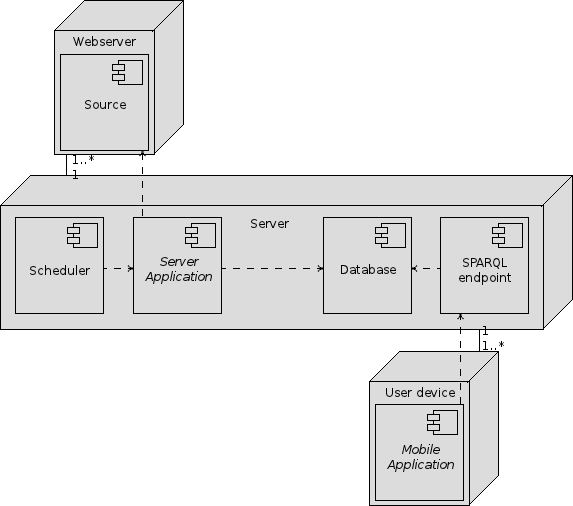
\includegraphics{./figures/deployment-s.png}
 % deployment-s.png: 573x506 pixel, 112dpi, 13.00x11.48 cm, bb=0 0 368 325
 \caption{Diagram nasazení serverové aplikace}
 \label{fig:server:deployment}
\end{figure}


\subsection{Použité technologie}
Mnoho použitých technologií bylo dáno zadáním práce, byl mi tak do značné míry usnadněn jejich výběr. Na druhou stranu nejsou dané technologie dokonalé, takže by často bývala práce s jinými snazší.

Celá serverová aplikace je napsána v \emph{JavaScriptu}, zprovozněna na \emph{Node.js}, datovým úložištěm se stalo \emph{MongoDB}.

\subsubsection{JavaScript}
Využití \emph{JavaScriptu} bylo pro svoje pravděpodobné vzrůstající nasazení v budoucnosti a své specifické vlastnosti dáno jako nefunkční požadavek.

\subsubsection{Node.js}
\emph{Node.js} (\url{http://nodejs.org/}) je platforma postavená nad běhovým prostředím JavaScriptu z Chrome. Slouží ke tvorbě rychlých, škálovatelných síťových aplikací. Node.js využívá událostmi řízený neblokovací I/O model, který ho činí nenáročným a efektivním, vhodným pro datově náročné \textit{real-timové} aplikace běžící v distribuovaném prostředí \cite{Node}.

Použití Node.js bylo vynuceno nefunkčním požadavkem, jednalo se ale o velmi cennou zkušenost -- je novou technologií a ačkoliv je jeho dokumentace na slušné úrovni, není zatím vytvořena dostatečně velká báze příkladů a nejlepších praktik, takže jsem se k nim musel postupně dostat a při té příležitosti se toho hodně naučil. Navíc, zdá se, se budou nabité vědomosti v budoucnu hodit.

\subsubsection{MongoDB}
\emph{MongoDB} (\url{http://www.mongodb.org/}) je škálovatelnou, vysoce výkonnou, otevřenou NoSQL databází napsanou v C++ \cite{Mongo}.

\subsubsection*{ }
Celé prostředí serverové aplikace je umístěno v serverové edici \glsname{GNU}/linuxové distribuce \emph{Ubuntu} (\url{http://www.ubuntu.com/}) a ta je pro snadnou přenositelnost nainstalována do kontejneru virtuálního stroje virtualizačního řešení \emph{VirtualBox} (\url{http://www.virtualbox.org/}).

\subsection{Použité knihovny}
Mimo standardního JavaScriptu lze v Node.js využívat i specifická rozšíření a množství modulů třetích stran. Z těch jsem využil:
\begin{itemize}
 \item \emph{date-utils} (\url{https://github.com/JerrySievert/node-date-utils}) -- mikro framework doplňující funkcionalitu JavaScriptového objektu Date. Zvažováno bylo i použití \emph{dateformat} (\url{https://github.com/felixge/node-dateformat}), ten je ale pro projekt méně vhodný. Oba moduly jsou stále ve vývoji.
 \item \emph{express} (\url{http://expressjs.com/}) -- renomovaný framework pro tvorbu webových aplikací založený na middleware frameworku \emph{connect} (\url{http://www.senchalabs.org/connect/}).
 \item \emph{iCalendar} (\url{https://github.com/tritech/node-icalendar}) -- knihovna pro práci s formátem iCalendar. Modul je stále ve vývoji. Zvažovány byly i další knihovny, například \emph{ical} (\url{https://github.com/peterbraden/node-ical}), ty ale implementovaly ještě méně možností, než použitá.
 \item \emph{iconv} (\url{https://github.com/bnoordhuis/node-iconv}) -- knihovna pro obsluhu systémového příkazu iconv sloužícímu k převádění kódování.
 \item \emph{jquery} (\url{https://github.com/coolaj86/node-jquery}) -- wrapper umožňující využít renomovanou JavaScriptovou knihovnu \emph{jQuery} (\url{http://jquery.com/}) v prostředí Node.js. Je zde využit \emph{jsdom} (\url{https://github.com/tmpvar/jsdom}) -- JavaScriptová implementace DOM.
 \item \emph{rdfstore} (\url{https://github.com/antoniogarrote/rdfstore-js}) -- JavaScriptová implementace \emph{\glsname{RDF}} grafového úložiště s podporou pro \emph{\glsname{SPARQL}}. Data mohou být (a v implementaci \glsname{DP} jsou) persistentně ukládána prostřednictvím Node.js modulu-ovladače \emph{mongodb} (\url{https://github.com/christkv/node-mongodb-native}) do NoSQL databáze \emph{MongoDB} (\url{http://www.mongodb.org/}). Modul je stále ve vývoji.
 \item \emph{soap} (\url{https://github.com/milewise/node-soap}) -- \todo{Pouze pokud se objeví podpora poskytnutého WSDL.}
\end{itemize}

\subsection{Použité nástroje}



\section{Mobilní aplikace}
\subsection{Potřeby uživatelů}
\subsubsection{Potřeba určit cílovou pozici}
\subsubsection{Potřeba určit aktuální pozici}
\todo{Seznam a popis jednotlivých potřeb uživatelů.}
% Tato sekce slouží jako seznam potřeb uživatelů, se kterými jsem se v průběhu práce setkal. Ne všechny potřeby byly později zapracovány do výsledné aplikace, některé totiž nebyly natolik důležité, aby se je vyplatilo v aplikaci mít a zastiňovat jimi potřeby důležitější. Další potřeby bývaly protichůdné a také je nešlo implementovat zároveň. Popisu uživatele se věnuje už sekce \ref{sec:popisUzivatele}.
% 
% \subsection{Potřeba se někam dostat}
% Touto potřebou se zabývá celá práce. Student zná označení místnosti (nebo i méně exaktní identifikátor), ale neví, kde se daná místnost nachází, ani kudy se k ní dostat. 
% 
% Hledaná místa mohou být různá, může to být třeba:
% \begin{itemize}
% \item učebna (ve které má student výuku nebo zkoušku),
% \item kancelář vyučujícího (ke kterému si jde pro známku z předmětu nebo na konzultaci),
% \item toalety (nejbližší nebo třeba nejméně frekventované),
% \item občerstvení (nejbližší automat nebo bufet s velkým sortimentem),
% \item hasící přístroj (jeho potřeba není častá, takže se jím dále nebudeme zabývat),
% \item únikový východ (také se jím, ze stejných důvodů, nebudeme zabývat),
% \item vrátnice (ta se ale hledá svou výlučnou přítomností u vchodu do budovy snadno),
% \item další takzvané body zájmu.
% \end{itemize}
% 
% Lokalizace hledaného místa může být provedena při znalosti:
% \begin{itemize}
% \item označení místnosti (KN:E-107), pokud hledáme učebnu a známe ho třeba z rozvrhu,
% \item starého označení (K1), pokud nám někdo řekne označení z doby před přečíslováním,
% \item oficiálního názvu místnosti (Zengerova posluchárna),
% \item neoficiálního názvu místnosti (Solárium, Bouračka, Bufet\dots),
% \item jména vyučujícího, pokud hledáme jeho kancelář,
% \item umístění vchodu do budovy, pokud třeba hledáme vrátnici,
% \item polohy všech míst, které přicházejí v úvahu (třeba bufetů), nebo to a navíc ještě
% \item přibližné aktuální polohy, pokud hledáme něco nejbližšího.
% \end{itemize}
% 
% \subsection{Potřeba určit polohu místa}
% Nejprve je nutné zjistit polohu místa, kam se potřebujeme dostat\footnote{Teoreticky je možné polohu neznat a tupě se řídit shora podávanými instrukcemi, toto řešení ale není lidské mentalitě příjemné a proto se jím práce nezabývá.} a až poté má smysl se zamýšlet nad samotnou cestou. Poloha se dá s předchozími zkušenostmi odhadnout,\footnote{Například poloha místnosti se dá odhadnout z jejího názvu, který sám o sobě identifikuje budovu a~podlaží.} předchozí zkušenosti ale nejsou zaručeny a správný odhad teprve ne.
% 
% K přesnému určení místa se dá dospět několika způsoby:
% \begin{itemize}
% \item náhodným zkoušením, to ale nebývá optimální,
% \item přeptáním se, to ale dělá, často introvertním, studentům problémy,
% \item vyhledáním v mapě, pokud je k dispozici.
% \end{itemize}
% 
% \subsection{Potřeba určit cestu k místu}
% Teprve tehdy, až známe polohu hledané místnosti, k ní můžeme začít určovat cestu. Způsoby jsou stejné jako u hledání místa samotného -- zkoušení, přeptávání a vyhledání na~mapě. 
% 
% \subsection{Potřeba navigační aplikace}
% Všechny předchozí potřeby by se daly uspokojit vhodnou aplikací -- ta dokáže určit polohu místa a nalézt k němu cestu pro uživatele velmi komfortně. Aplikaci je nicméně potřeba vytvořit a je potřeba to udělat pořádně -- tím se zabývají následující potřeby, jinak bude pro~uživatele lepší se i nadále spoléhat na svou intuici.
% 
% \subsection{Potřeba mobilní aplikace}
% Místnost je dost často potřeba najít okamžitě, několik minut předtím, než v ní máme být. V této době není čas shánět se po počítači, navíc už můžeme být v pohybu předpokládaným směrem. Z toho plyne potřeba aplikace mobilní.
% 
% Studenti Fakulty elektrotechnické, kterými se práce zabývá, zpravidla tíhnou k technickým hračkám, například k mobilním telefonům a tím pádem i jejich aplikacím, více, než většina populace. Dá se tedy předpokládat, že mobilní telefony mají, a dá se předpokládat i~to, že budou tyto telefony schopny provozovat jednoduchou navigační aplikaci.
% 
% \subsection{Potřeba použitelné aplikace}
% Aby aplikaci vůbec někdo používal, je nutné, aby byla použitelná, aby se s ní dalo pracovat i bez návodu a vše bylo přehledné. Je dobré, když aplikace umožňuje vyhledávat i~bez diakritiky, nerozlišuje při vyhledávání velikost písmen, umožní zadat regulární výraz pro~nalezení místa s ne úplně přesně známým názvem a podobně.
% 
% \subsection{Potřeba korespondující navigace aplikace se skutečností}
% Je nutné, aby se dokázal uživatel podle aplikace někam dostat. Musí se nejprve zorientovat, zjistit kam se chce dostat a kudy se tam dostat. V těchto krocích mu musí aplikace pomáhat.
% 
% \subsection{Potřeba multiplatformní aplikace}
% Mobilní zařízení jsou specifická svými implementacemi standardů, dost často jsou tyto implementace, pokud jsou vůbec přítomny, pro nedostatek prostředků poskytovaných zařízením osekané a někdy i od standardů odlišné. Není to ideální, ale je to pochopitelné. Bohužel je ale nepřeberné množství zařízení a téměř u každého modelu je něco jinak, než jinde. Je pak v některých případech velmi těžké nalézt multiplatformní řešení.
% 
% \subsection{Potřeba aktuálního obsahu aplikace}
% Obsah aplikace by měl být aktuální a reflektovat stávající situaci: uzavírky, přestavby a~jiné mimořádné události. Aplikace může čerpat některá aktuální data z \url{http://udb.feld.cvut.cz}, například označení místnosti, ve které má student podle rozvrhu následující hodinu, nebo kanceláře vyučujícího. Navede-li aplikace někoho špatně, aktuálně opravovanou, slepou cestou, riskuje se ztráta uživatele.
% 
% \subsection{Potřeba offline provozu aplikace}
% Částečně v rozporu s předchozím bodem je potřeba offline provozu aplikace. Mnoho studentů ještě nemá ve svých mobilních zařízeních možnost připojení k Internetu a o ty by aplikace online provozem přišla. Aplikace by tedy měla zvládat práci offline, ale také by mohla umožňovat online provoz a aktualizace pro offline provoz.
% 
% \subsection{Potřeba navedení optimální cestou aplikací}
% \label{subs:UNcestaAplikaci}
% Hledání optimální cesty je poměrně složitá záležitost, ačkoliv se to na první pohled nezdá. Optimální cesta není ta nejkratší nebo nejrychlejší, je to mnohem složitější. Do hry vstupuje mnoho kritérií, například:
% \begin{itemize}
% \item délka cesty -- má být většinou nejkratší,
% \item doba cesty -- má být většinou nejkratší,
% \item terén -- tady už začínají komplikace, někdo se rád projde po schodech, jiný může mít zlámanou nohu, tak chce jet páternosterem a další je na vozíčku, předchozí způsoby nemůže využít a musí jet obyčejným výtahem,
% \item zapamatovatelnost cesty -- má být většinou nejsnazší,
% \item frekventovanost -- někteří se rušným cestám vyhýbají, jiní je vyhledávají,
% \item místa kolem cesty -- někteří raději nevolí cestu kolem kanceláří neoblíbených vyučujících...
% \end{itemize}
% Na první pohled je jasné, že téměř nikdy nemůže existovat cesta, která by byla ve všech zmiňovaných kritériích nejlepší. Je nevděčné vytvářet univerzálně nejlepší cestu a nad lidské síly sestavovat optimální algoritmus pro zjištění individuálně nejlepší cesty; vytvořit použitelnou implementaci v omezeném mobilním prostředí tedy bohužel asi nepůjde.
% 
% \subsection{Potřeby návštěvníků na aplikaci}
% Návštěvníci mají specifické potřeby na aplikaci. Zajímavé by mohlo třeba být prozkoumat potřeby potencionálních studentů, kteří se jdou podívat na den otevřených dveří, a~poskytnout jim aplikaci jako průvodce mezi jednotlivými stanovišti dne otevřených dveří. Zadání práce ale vymezuje cílovou skupinu jako studenty FELu, takže se těmito potřebami nebudeme dále zabývat.
% 
% 
% 
\subsection{Prototypy}
\todo{Pojednání o vytvořených prototypech, možná nakonec pod něco zařadím, nebude mít velký rozsah.}
% Po ujasnění několika základních potřeb a požadavků jsem začal vytvářet prototypy. Nejprve pouze jednoduché low fidelity prototypy pro vyjasnění základních požadavků, později sofistikovanější high fidelity prototypy reprezentující chování i vzhled výsledné aplikace.
% 
% \subsection{Low fidelity prototypy}
% Low fidelity prototypy jsou, většinou papírové, snadno vytvořitelné prototypy, na kterých se navrhují a testují některé základní aspekty aplikace -- rozvržení komponent, jednoduchá interakce, návaznost akcí a podobně. Mají tu výhodu, že zadavateli přiblíží finální aplikaci, udělá si konkrétnější představu a lépe se mu pak formulují požadavky.
% 
% Za pomoci low fidelity prototypů se vymezily jednotlivé obrazovky aplikace. Výchozí obrazovka je v podstatě jedinou nutnou obrazovkou aplikace, obsahuje menu pro přechod do dalších obrazovek, vyhledávací formulář a krátkou nápovědu. Dalšími obrazovkami jsou nápověda, nápověda regulárních výrazů a obrazovka se základními informacemi o programu.
% 
% Nejvýznamnějším ovládacím prvkem bude velké vyhledávací pole uprostřed úvodní obrazovky -- uživatel zde bude moci zadat všechno, co potřebuje nalézt, a aplikace by mu to měla vyhledat. V případě, že bude nalezeno více výsledků, zobrazí se jejich seznam (viz obrázek~\ref{fig:LFviceVysledku}\footnote{Low fidelity prototypy byly vytvořeny v nástroji Balsamiq Mockups \cite{BalsamiqMockups}.}), ze kterého si bude moci uživatel vybrat nebo upřesnit hledaný výraz, jinak se navede rovnou k cíli (viz obrázek~\ref{fig:LFjedinyVysledek}).
% 
% \begin{figure}[ht]
% \begin{center}
% 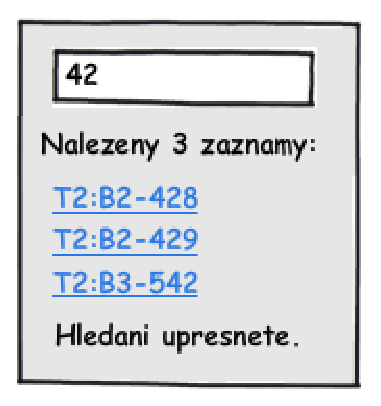
\includegraphics[width=30mm]{figures/LFviceVysledku}
% \caption{Nalezení několika výsledků}
% \label{fig:LFviceVysledku}
% \end{center}
% \end{figure}
% 
% \begin{figure}[ht]
% \begin{center}
% 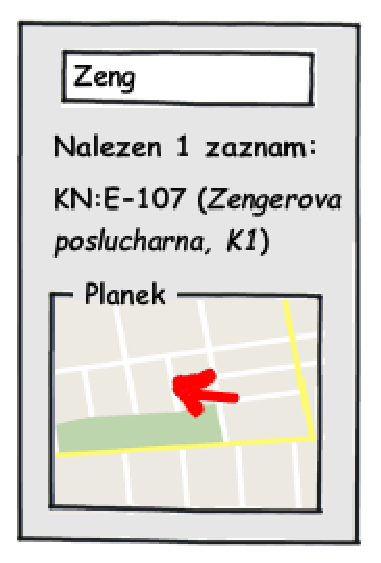
\includegraphics[width=30mm]{figures/LFjedinyVysledek}
% \caption{Nalezení jediného výsledku}
% \label{fig:LFjedinyVysledek}
% \end{center}
% \end{figure}
% 
% Aplikace by ještě měla poskytovat rozšířené vyhledávání s upřesněním hledaných míst a~zadáním výchozího bodu.
% 
% \noindent\textbf{Ostatní low fidelity prototypy jsou na přiloženém CD.}
% 
% 
% 
% \subsection{High fidelit prototyp}
% High fidelity prototypy jsou už sofistikovanějšími prototypy, jejich vytvoření tudíž trvá déle, ale přesto se je vyplatí udělat před finální aplikací -- nemají totiž plnou funkčnost konečné aplikace, nemusí ošetřovat vstupy a řešit nestandardní situace, takže se pořád vytvoří relativně rychle, přičemž už zadavateli dokáží realisticky demonstrovat finální práci s aplikací.
% 
% High fidelity prototyp jsem vytvořil pomocí XHTML, ECMAScriptu a CSS. Jedná se o~velmi vhodné technologie pro tvorbu prototypů -- rychle se vytvoří a snadno se pak upravují. Testování takto vytvořených prototypů je také příjemné -- v případě v prototypu nevyřešené situace lze snadno připravit výslednou situaci a testerovi ji na dálku bez nějakých komplikací podstrčit.
% 
% Na obrázku \ref{fig:HFviceVysledku} je vidět high fidelity prototyp ve stavu zobrazení více výsledků vyhledání.
% 
% \begin{figure}[ht]
% \begin{center}
% 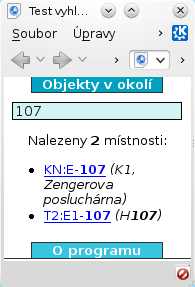
\includegraphics[width=30mm]{figures/HFviceVysledku}
% \caption{Nalezení několika výsledku}
% \label{fig:HFviceVysledku}
% \end{center}
% \end{figure}
% 
% Testování high fidelity prototypů je hlouběji popisované v kapitole o testování (viz \ref{sec:testhfp}).
% 
% \noindent\textbf{High fidelity prototyp je na přiloženém CD.}
% 
% 
% 
\subsection{Případy užití}
\todo{Různé případy užití v textové formě.}
% Případy užití (use cases) jsou scénáře popisující chování systému z pohledu vnějšího aktéra. Případy užití vymezují, kdo a co bude jak dělat a z tohoto základu se později sestaví funkční požadavky. Už ze zadání aplikace vyplývá potřeba jediného aktéra -- studenta. Základní případy užití jsou následující:
% \subsection{UC1: Hledání místnosti podle označení}
% \label{ssec:UChledaniMistnosti}
% \begin{description}
% \item[Aktéři:] Student.
% \item[Systém:] Navigační aplikace.
% \item[Vstupní podmínky:] ~\\*[-1.5em]
%  \begin{itemize}
%  \item Student je ve výchozí obrazovce aplikace.
%  \item Student se chce dostat do místnosti KN:E-9.
%  \end{itemize}
% \pagebreak
% \item[Hlavní scénář:] ~\\*[-1.5em]
%  \begin{enumerate}
%  \item Student vstoupí do vyhledávacího formuláře.
%  \item Student zadá písmeno \emph{K}.
%  \item Aplikace zobrazí seznam místností obsahujících písmeno \emph{K}.
%  \item Student zadá písmeno \emph{N}.
%  \item Aplikace zobrazí seznam místností obsahujících výraz \emph{KN}.
%  \item Student postupně zadá znaky \emph{:E-} a aplikace zúží seznam.
%  \item Student zadá číslici \emph{9}.
%  \item Aplikace zobrazí plán cílového patra s vyznačeným cílem.
%  \item Student dojde podle plánu k cíli.
%  \end{enumerate}
% \item[Poznámky:] ~\\*[-1.5em]
%  \begin{itemize}
%  \item Místnost by mělo jít stejným způsobem vyhledat i podle starého číslování a zažitých názvů.
%  \item Při zadání dvou a méně znaků lze kvůli nízkému výkonu zařízení a zachování přehlednosti zobrazovat upozornění na nutnost zadání více znaků.
%  \end{itemize}
% \end{description}
% 
% \subsection{UC2: Hledání neexistující místnosti}
% \begin{description}
% \item[Aktéři:] Student.
% \item[Systém:] Navigační aplikace.
% \item[Vstupní podmínky:] ~\\*[-1.5em]
%  \begin{itemize}
%  \item Student je ve výchozí obrazovce aplikace.
%  \item Student se chce dostat do místnosti KN:X-777.
%  \end{itemize}
% \item[Hlavní scénář:] ~\\*[-1.5em]
%  \begin{enumerate}
%  \item Student vstoupí do vyhledávacího formuláře.
%  \item Student postupně zadá znaky \emph{KN:X}.
%  \item Aplikace sdělí studentovi, že místnost neexistuje.
%  \end{enumerate}
% \item[Poznámky:] ~\\*[-1.5em]
%  \begin{itemize}
%  \item Podrobný popis postupu zadávání znaků a reakcí aplikace je v UC1 \ref{ssec:UChledaniMistnosti}.
%  \end{itemize}
% \end{description}
% 
% \pagebreak
% \subsection{UC3: Hledání kanceláře podle jména sídlícího vyučujícího}
% \begin{description}
% \item[Aktéři:] Student.
% \item[Systém:] Navigační aplikace.
% \item[Vstupní podmínky:] ~\\*[-1.5em]
%  \begin{itemize}
%  \item Student je ve výchozí obrazovce aplikace.
%  \item Student chce nalézt kancelář Zdeňka Míkovce.
%  \end{itemize}
% \item[Hlavní scénář:] ~\\*[-1.5em]
%  \begin{enumerate}
%  \item Student vstoupí do vyhledávacího formuláře.
%  \item Student zadá písmeno \emph{M}.
%  \item Aplikace zobrazí seznam místností obsahujících písmeno \emph{M}.
%  \item Student zadá písmeno \emph{í}.
%  \item Aplikace zobrazí seznam místností obsahujících výraz \emph{Mí}.
%  \item Student zadá písmeno \emph{k}.
%  \item Aplikace zobrazí plán cílového patra s vyznačeným cílem.
%  \item Student dojde podle plánu k cíli.
%  \end{enumerate}
% \end{description}
% 
% \subsection{UC4: Hledání nejbližšího nápojového automatu}
% \begin{description}
% \item[Aktéři:] Student.
% \item[Systém:] Navigační aplikace.
% \item[Vstupní podmínky:] ~\\*[-1.5em]
%  \begin{itemize}
%  \item Student je ve výchozí obrazovce aplikace.
%  \item Student se chce dostat k nejbližšímu nápojovému automatu.
%  \item Student se nachází před místností KN:E-9.
%  \end{itemize}
% \item[Hlavní scénář:] ~\\*[-1.5em]
%  \begin{enumerate}
%  \item Student vstoupí do vyhledávacího formuláře.
%  \item Student vyhledá místnost KN:E-9 podle UC1 \ref{ssec:UChledaniMistnosti}.
%  \item Aplikace zobrazí plán cílového patra s vyznačeným výchozím místem.
%  \item Student v plánu vyhledá požadovaný nápojový automat.
%  \item Student dojde podle plánu k cíli.
%  \end{enumerate}
% \end{description}
% 
% \subsection{UC5: Hledání za pomoci regulárních výrazů}
% \begin{description}
% \item[Aktéři:] Student.
% \item[Systém:] Navigační aplikace.
% \item[Vstupní podmínky:] ~\\*[-1.5em]
%  \begin{itemize}
%  \item Student je ve výchozí obrazovce aplikace.
%  \item Student se chce dostat do místnosti KN:E-9.
%  \end{itemize}
% \item[Hlavní scénář:] ~\\*[-1.5em]
%  \begin{enumerate}
%  \item Student vstoupí do vyhledávacího formuláře.
%  \item Student zadá znak \emph{-}.
%  \item Aplikace zobrazí seznam místností obsahujících znak \emph{-}.
%  \item Student zadá číslici \emph{9}.
%  \item Aplikace zobrazí seznam místností obsahujících výraz \emph{-9}.
%  \item Student zadá znak \emph{\$}.
%  \item Aplikace zobrazí seznam místností končících výrazem \emph{-9}.
%  \item Student si vybere ze seznamu místnost KN:E-9.
%  \item Aplikace zobrazí plán cílového patra s vyznačeným cílem.
%  \item Student dojde podle plánu k cíli.
%  \end{enumerate}
% \end{description}


\subsection{Funkční požadavky}
Funkčními požadavky (\textit{functional requirements}) jsou myšleny takové požadavky, které jsou zaměřeny na jednotlivé funkcionality. Pro mobilní aplikaci mezi ně patří především:

\begin{enumerate}
 \item Aplikace umožní pokročilému uživateli zadat vlastní \glsname{SPARQL} dotaz. Ten se odešle na server, kde se zpracuje, a výslek se navrátí uživateli.
 \item Pro méně znalé uživatele \glsname{SPARQL} a pro uživatele minimalizující použití klávesnice vytvořte předpřipravené dotazy pro základní scénáře použití aplikace.
 \item Implementujte funkcionalitu umožňující určení aktuální pozice a její předání dalšímu zpracování.
 \item Aplikace dokáže na mapě vizualizovat určitou pozici.
%  \item Aplikace umožní vizualizovat polohu uživatele na základě GPS souřadnic.
%  \item Aplikace umožní vizualizovat polohu uživatele na základě známého blízkého objektu (např. čísla místnosti).
%  \item Aplikace umožní vizualizovat polohu hledaného objektu.
 \item Aplikace dokáže vizualizovat \glsname{HTML} data nebo data jako \glsname{HTML}.
 \item Aplikace bude poskytovat nápovědu pro snazší použití.
 \item Aplikace bude postavená nad daty reprezentovanými výše uvedenou ontologií.
\end{enumerate}

% \subsection{FR-M-1: Možnost vlastních \emph{SPARQL} dotazů}
% Aplikace umožní pokročilému uživateli zadat vlastní \emph{SPARQL} dotaz. Ten se odešle na server, kde se zpracuje, a výslek se navrátí uživateli.
% \subsection{FR-M-2: Výběr předpřipravených dotazů}
% Pro méně znalé uživatele \emph{SPARQL} a pro uživatele minimalizující použití klávesnice vytvořte předpřipravené dotazy pro základní scénáře použití aplikace.
% % \subsection{FR-M-: Vyhledání místností}
% % Připravte aplikaci mimo předem nespecifických dotazů i na ty požadující vyhledání místností. 
% % \subsection{FR-M-: Vyhledání bodů zájmu}
% % Připravte aplikaci mimo předem nespecifických dotazů i na ty požadující vyhledání bodů zájmu. 
% \subsection{FR-M-3: Určení aktuální pozice}
% Implementujte funkcionalitu umožňující určení aktuální pozice a její předání dalšímu zpracování.
% \subsection{FR-M-4: Vizualizace pozice}
% Aplikace dokáže na mapě vizualizovat určitou pozici.
% \subsection{FR-M-5: Vizualizace \emph{HTML} dat}
% Aplikace dokáže vizualizovat \emph{HTML} data nebo data jako \emph{HTML}.
% \subsection{FR-M-6: Nápověda}
% Aplikace bude poskytovat nápovědu pro snazší použití.


\subsection{Nefunkční požadavky}
Nefunkčními požadavky (\textit{non-functional requirements}) jsou myšleny takové požadavky, které jsou zaměřeny na dílo jako celek, nikoliv na jednotlivé funkcionality. Pro mobilní aplikaci mezi ně patří především:

\begin{enumerate}
 \item Aplikaci vytvořte v \glsname{HTML}5, aby byla na současných, obzvláště mobilních, zařízeních multiplatformní.
 \item Aplikace bude funkční v prohlížečích na nejnovějších verzích \glsname{OS} Android, iOS a Symbian.
 \item Aplikace bude funkční v majoritních desktopových prohlížečích.
 \item Při vývoji se zaměřte i na použitelnost, aplikaci by měl být schopný, po krátkém zaškolení, používat jakýkoliv běžný student Fakulty informačních technologií.
 \item Snažte se nabízet alternativy k zadávání dlouhých textů, aby byla usnadněna obsluha uživatelům mobilních zařízení bez hardwarových klávesnic.
 \item Práce nemusí nutně obsáhnout celou zpracovávanou doménu, je ale žádané, aby kvalitně zpracovala hlavní scénáře využití a nebránila dalšímu rozšiřování.
 \item Zveřejněte aplikaci a její data pod svobodnými licencemi z rodin \glsname{GNU}, \emph{Creative Commons} a kompatibilními, aby byl umožněn další rozvoj nezávislý na původním autorovi.
 \item Aplikace umožní využití off-line. \todo{Vynechám -- muselo by se složitě indexovat.}
\end{enumerate}


% \subsection{NFR-M-1: Multiplatformnost}
% Aplikaci vytvořte v \emph{HTML5}, aby byla na současných, obzvláště mobilních, zařízeních co nejvíce multiplatformní. Bude funkční minimálně v nejnovějších verzích OS Android, iOS a Symbian.
% \subsection{NFR-M-2: Použitelnost}
% Při vývoji se zaměřte i na použitelnost, aplikaci by měl být schopný, po krátkém zaškolení, používat jakýkoliv běžný student Fakulty informačních technologií.
% \subsection{NFR-M-3: Omezené použití klávesnice}
% Snažte se nabízet alternativy k zadávání dlouhých textů, aby byla usnadněna obsluha uživatelům mobilních zařízení bez hardwarových klávesnic.
% % \subsection{NFR-M-: Offline provoz}
% \subsection{NFR-M-4: Dejte přednost kvalitě zpracování}
% Práce nemusí nutně obsáhnout celou zpracovávanou doménu, je ale žádané, aby kvalitně zpracovala hlavní scénáře využití a nebránila dalšímu rozšiřování.
% \subsection{NFR-M-5: Svobodné licence}
% Zveřejněte aplikaci a její data pod svobodnými licencemi z rodin \emph{GNU}, \emph{Creative Commons} a kompatibilními, aby byl umožněn další rozvoj nezávislý na původním autorovi.


\subsection{Návrh řešení}
\todo{Diskuse alternativ.}

\todo{Volba implementačního prostředí.}

\todo{Struktura.}

% Návrh (design) této aplikace neprobíhal příliš dlouho, aplikace nemá být nijak složitá a~rozsáhlá, ani není po stránce návrhu nějak výjimečná, takže se zde návrhu příliš věnovat nebudeme.
% 
% \subsection{Vyhledávání}
% Stěžejní funkcí má být vyhledávání, to je zároveň i stěžejním bodem návrhu. Je nutné splnit všechny funkční i nefunkční požadavky, kde je vyhledávání silně zastoupeno.
% 
% Vyhledávací algoritmus by měl fungovat následovně, začnu popisovat od databáze, ze které se vyhledává. Databáze bude obsahovat mnoho (až tisíce) záznamů a je proto v mobilním prostředí nutné, aby bylo vyhledávání, včetně samotné databáze, optimalizované. Aby došlo v průběhu vyhledávání ke snížení toku dat algoritmem, provedeme dekompozici databáze a vyčleníme hledatelné položky (označení učeben, jména vyučujících...) stranou, můžeme je ještě abecedně seřadit. Tady optimalizace databáze prozatím končí a můžeme se přesunout k samotnému algoritmu.
% 
% Původně jsem zamýšlel vyhledávat binárním půlením nebo jiným algoritmem optimalizovaným pro seřazený seznam, přišel ale požadavek na vyhledávání pomocí regulárních výrazů a tím tato možnost odpadla -- je potřeba projít všechny místnosti a zkontrolovat každou položku.
% 
% Regulární výrazy se nám většinou postarají i o nerozlišování velikosti písmen, takže si jimi alespoň pomůžeme k dalšímu požadavku.
% 
% Při kontrole položky můžeme zároveň vyřešit i požadavek na hledání bez diakritiky, zase ale musíme optimalizovat. Nebylo by složité vytvořit algoritmus, který zkouší nahradit každé písmeno bez diakritiky jeho diakritickými variantami, tím by nám ale výrazně narostla náročnost algoritmu, slovo \emph{mistnost} by tak najednou odpovídalo sto dvaceti osmi výrazům (\emph{mistnost}, \emph{m\textbf{í}stnost}, \emph{mi\textbf{š}tnost}, \emph{m\textbf{íš}tnost}...), tolikrát ale nezvládneme se současným výkonem mobilních zařízení celou databázi prohledat.\footnote{V praxi není toto omezení tolik markantní, označení místností obsahuje spíše znaky bez diakritiky. Vyhledávané osoby ale diakritiku ve jménech mají, takže toto omezení zachováme.} Umožníme vyhledávat buď jen s diakritikou, nebo bez, čímž slovo \emph{mistnost} bude odpovídat pouze dvěma výrazům (\emph{mistnost} a \emph{m\textbf{í}stnost}). Vyřešíme to následovně, všechny diakritiku obsahující položky v již dříve zmíněném duplicitním seznamu uložíme do tohoto seznamu ještě jednou, tentokrát bez diakritiky.
% 
% Nalezeným položkám přiřadíme místnosti, které reprezentují (například položce \emph{Josef Vomáčka} místnost \emph{KN:E-108}), vyřadíme duplicitní místnosti a seřadíme je podle abecedy.
% 
% \subsection{Navigace}
% Zpočátku jsme v analýze uvažovali o vyznačení cesty z výchozího bodu do cílového, to by ale, mimo náročného algoritmu, dost uživateli v některých věcech přitížilo. V první řadě by přišel o mnoho místa malého displeje formulářem pro zadání výchozího bodu, v druhé řadě by bylo vytvoření optimálního algoritmu hledajícího cestu pravděpodobně nemožné (viz \ref{subs:UNcestaAplikaci}) a špatná cesta by se uživateli nemusela líbit. Problém v tom naštěstí pravděpodobně nebude, budovy nejsou stavěné jako bludiště a navigace po nich s plánkem není problém.
% 
% Vyhledáním místnosti získá aplikace cíl, ke kterému je potřeba uživatele navést. Dobrým řešením je ukázat uživateli plán cílového patra s vyznačeným cílem, orientačními body, schodišti (a výtahy) a vstupy do budovy (s~rozdíly pater). Uživatel se tak dokáže v plánu zorientovat, i kdyby se mu to doposud nepodařilo, schodiště (většinou vedou budovou každým patrem) a vchody do budovy (většinou jsou maximálně dva) k tomu velmi pomohou. Plán pouze cílového patra proto, že cestu po schodech nemá cenu vizualizovat (dokonce je to spíše nevhodné) a v rámci výchozího patra je většinou zcela zřejmé, jak se ke schodům dostat. Uživatel se tedy zvládne dostat do uvedeného patra a tam už podle plánu k hledané místnosti sám bez větších komplikací.

\subsection{Návrh bezpečnosti}
\todo{Injekce JS, ošetření vstupů, white-listing URL, elementů, atributů, zakázání cizích zdrojů...}

\subsection{Návrh nasazení}
Nasazení mobilní aplikace bylo navrženo tak, jak je vidět na obrázku \ref{fig:mobile:deployment}. Aplikace komunikuje se \glsname{SPARQL} endpointem serverové aplikace, v případě neposkytování daných informací aplikace komunikuje přímo se zdrojem informací.
\begin{figure}[h]
 \centering
 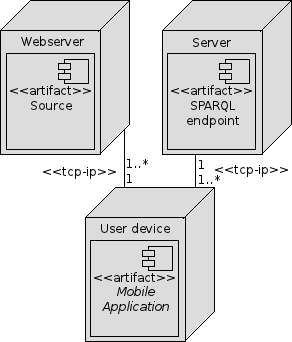
\includegraphics{./figures/deployment-m.png}
 \caption{Diagram nasazení mobilní aplikace}
 \label{fig:mobile:deployment}
\end{figure}


\subsection{Použité technologie}
Níže uvádím soupis použitých technologií s odůvodněním, proč byly vybrány a v jakém kontextu použity.

\subsubsection{HTML5}
Většina technologií tvořících mobilní aplikaci by se dala zahrnout do pojmu HTML5 (v širším smyslu významu). Pomocí JavaScriptu se manipuluje s \glsname{HTML} strukturou, která je prezentována za pomocí \glsname{CSS}, klíčová část aplikace -- mapa -- je tvořena \glsname{SVG} (o tom ještě dále). Technologie byly vybrány pro jejich výbornou portovatelnost -- téměř všechna dnešní zařízení je implementují podobně (nebo alespoň mají takové výkonnostní parametry, že na nich lze provozovat přidanou vrstvu abstrahující od skutečné implementace).

\subsubsection{SVG}
Mapa použitá v aplikaci je implementována prostřednictvím \glsname{SVG}. Rozhodnutí bylo učiněno na základě identifikace a porovnání možných technologií:
\begin{itemize}
 \item Statické obrázky s předgenerovanými proměnnými částmi.
 \item Statické obrázky s dynamicky pozicovanými proměnnými částmi.
 \item Dynamicky kreslené obrázky na \textit{canvas}.
 \item Statické \glsname{SVG} s dynamickými úpravami.
\end{itemize}

První zmíněné řešení bylo zavrženo kvůli nízké flexibilitě -- není možné dopředu vygenerovat všechny varianty obrázků, které by pokrývaly možné situace -- i kdyby to možné bylo, množství obrázků by bylo velmi vysoké\footnote{Pro pokrytí všech situací by byly třeba zvlášť obrázky s vyznačením kterékoliv místnosti, kteréhokoliv bodu zájmu, kterékoliv výchozí pozice\dots Vzhledem k rozsáhlosti mapy by tak počet obrázků byl enormní.} a pro omezenou paměťovou kapacitu cílových zařízení nevhodné.

Druhý přístup, dynamické pozicování, byl zavržen z důvodů optimalizací rozvržení prvků mobilními prohlížeči -- není zaručené, že se prvek (například ukazatel nalezené místnosti) skutečně umístí, kam má.

Nová vlastnost HTML5, kreslení prostřednictvím JavaScriptu na \textit{canvas} element, byla, narozdíl od předchozích možností, zvažována až do finálního rozhodnutí -- ačkoliv se jedná o řešení čistě v režii již používaných technologií (JavaScript, HTML), jeho využití jsem z několika důvodů zavrhl:
\begin{itemize}
 \item Neumožňuje nakreslený obrázek nijak upravit (například posunout ukazatel na mapě), ale musí se vždy překreslit, což je náročnější na zdroje.
 \item Kvůli principu dynamického generovaní obrázků JavaScriptem nelze kostru připravit pomocí běžných grafických editorů.
 \item Subjektivně mi přijde práce s mapou jako \glsname{SVG} obrázkem reprezentovaným \glsname{XML} dokumentem majícím \glsname{DOM} přehlednější, než s méně strukturovatelným JavaScriptem.
\end{itemize}

Reprezentaci mapy jsem tedy svěřil \glsname{SVG} z následujících důvodů:
\begin{itemize}
 \item Snadné vytvoření mapy prostřednictvím běžného grafického editoru.
 \item Možnost znovupoužití mapy standardního grafického formátu i v jiných projektech.
 \item Práce s mapou (něpř. vyznačování pozic) se provádí pouhodou úpravou jejího \glsname{DOM}.
 \item I po úpravách se stále jedná o týž objekt -- není nutné ho překreslovat.
\end{itemize}

Nutno podotknout, že jsou implementace kreslení na \textit{canvas} a \glsname{SVG} na různých mobilních zařízeních na různých úrovních, ani jedna ovšem nemá výrazně navrch \cite{CanIUse} \cite{MobileHtml}.

\subsubsection{PHP}
Z důvodů popsaných v podsekci \ref{sec:cross-origin} (str. \pageref{sec:cross-origin}) bylo nutné vytvořit podpůrnou serverovou aplikaci -- proxy. Po úvaze jsem se rozhodl pro využití jazyka \glsname{PHP}, který je podporovaný jako jediný nástroj pro tvorbu dynmického obsahu na fakultním webovém serveru \url{http://webdev.fit.cvut.cz/}. Tuto kombinaci, vzhledem k její podpoře ze strany fakulty a určení práce pro fakulní nasazení, považuji i přes jinde využitý JavaScript za vhodnou.


\subsection{Použité knihovny}
V práci byla, po úvaze, nakonec využita i práce třetích stran -- svobodné knihovny \emph{jQuery} a \emph{HTML Purifier}. Jejich krátký popis a odůvodnění následují:

\subsubsection{jQuery}
A

\subsubsection{HTML Purifier}
Po několika vlastních implementacích nástroje na pročištění a ošetření \glsname{HTML} vstupů pocházejících od třetích stran jsem sáhl k implementaci již prověřené -- oblast ošetření aplikace před škodlivými vstupy má z hlediska bezpečnosti vysokou prioritu a neustále se objevující nové hrozby nakonec vedly k tomu, že jsem se rozhodl nespoléhat na své vlastní implementace a využít \textit{know-how} tvůrců svobodné \glsname{PHP} knihovny  HTML Purifier (\url{http://htmlpurifier.org/}) -- ta odstraní případná nebezpečí za využití pokročilého auditovaného \textit{whitelistu} a v případě potřeby navíc zajistí validitu kódu. Knihovna je využita v rámci proxy zmíněné v předchozím odstavci.


\subsection{Použité nástroje}
Pro tvorbu aplikace byly použity převážně následující nástroje. Majorita jich je uvolněných pod svobodmými licencemi, zpravidla \glsname{GNU} \glsname{GPL} nebo kompatibilními. Jedinou výjimkou jsou některé mobilní prohlížeče, které byly použity k testování aplikace.

\subsubsection{Kate}
Většina práce, včetně mobilní aplikace, byla vytvořena v textovém editoru \glsname{Kate} (\url{http://kate-editor.org/}). Jedná se o velmi pokročilý nástroj pro práci s textem z prostředí \glsname{GNU}/Linuxového desktopového prostředí \glsname{KDE}. \glsname{Kate} nabízí zvýrazňování syntaxe všech v diplomové práci použitých formátů, poskytuje velmi užitečnou práci s regulárními výrazy, umožňuje pracovat s mnoha soubory najednou a, co je asi nejpodstatnější, plně se integruje do \glsname{KDE}, takže ním například lze prostřednictvím \gls{KIO} transparentně pracovat se vzdálenými soubory. \glsname{Kate} neumožňuje automatické doplňování kódu, nabízí ale již použitá slova kdekoliv v dokumentu, což je vlastnost v některých případech i lepší. Kate byl zvolen na základě velice kladných zkušeností pro napsání kódu v JavaScriptu, \gls{HTML}, \gls{CSS} i úpravy mapy v \gls{SVG}.

\subsubsection{Inkscape}
Grafické podklady práce byly vytvořeny v editoru vektorové grafiky Inkscape (\url{http://www.inkscape.org/}). Nástroj implementuje téměř kompletní specifikaci formátu \glsname{SVG} verze 1.1, je multiplatformní a svobodný. Inkscape byl vybrán kvůli předchozím výborným zkušenostem s prací v něm a vhodnosti pro tvorbu mapových podkladů.

\subsubsection{Kompare}
V případě potřeby důkladného porovnání souborů byl použit Kompare (\url{http://www.caffeinated.me.uk/kompare/}). Nástroj umožňuje velmi přehledně porovnat mimo jednotlivých souborů i celé jejich adresáře. Kompare neporovnává soubory sám, ale je nadstavbou nad konzolovou aplikací diff či obdobnou.

\subsubsection{Webové prohlížeče}
Aplikace byla průběžně testována v různých mobilních prohlížečích:
\begin{itemize}
 \item Mozilla Firefox (\url{http://www.mozilla.org/firefox}).
 \item Chromium (\url{http://chromium.org/}).
 \item rekonq (\url{http://rekonq.kde.org/}).
 \item Prohlížeč platformy Android (\url{http://www.android.com/}).
 \item Google Chrome for Android (\url{https://www.google.com/intl/en/chrome/android/}).
 \item Opera Mobile (\url{http://www.opera.com/mobile}).
 \item Internet Explorer Mobile (\url{http://www.microsoft.com/windowsphone/en-us/features/default.aspx#internet-explorer}).
Před dokončením byla navíc otestována panem inženýrem Havrylukem, vedoucím práce, v následujících prohlížečích:
 \item Nokia Browser for Symbian  (\url{http://browser.nokia.com/}).
 \item Prohlížeč platformy BlackBerry (\url{http://us.blackberry.com/smartphones/features/internet.jsp}).
 \item Safari (\url{http://www.apple.com/safari/}).
\end{itemize}

\subsubsection{Git}
Práce byla průběžně verzována systémem pro správu verzí Git (\url{http://git\-scm.com/}), čímž bylo zajištěné pohodlné zálohování jak ve smyslu možnosti návratu k některé z minulých verzí, tak i ve smyslu vzdáleného duplikování na serveru GitHub (\url{http://github.com/}). Pozitivním vedlejším efektem tohoto přístupu je možnost sledování vývoje prostřednictvím veřejného repozitáře.